% Options for packages loaded elsewhere
\PassOptionsToPackage{unicode}{hyperref}
\PassOptionsToPackage{hyphens}{url}
%
\documentclass[
  brazil,
]{book}
\usepackage{lmodern}
\usepackage{amssymb,amsmath}
\usepackage{ifxetex,ifluatex}
\ifnum 0\ifxetex 1\fi\ifluatex 1\fi=0 % if pdftex
  \usepackage[T1]{fontenc}
  \usepackage[utf8]{inputenc}
  \usepackage{textcomp} % provide euro and other symbols
\else % if luatex or xetex
  \usepackage{unicode-math}
  \defaultfontfeatures{Scale=MatchLowercase}
  \defaultfontfeatures[\rmfamily]{Ligatures=TeX,Scale=1}
\fi
% Use upquote if available, for straight quotes in verbatim environments
\IfFileExists{upquote.sty}{\usepackage{upquote}}{}
\IfFileExists{microtype.sty}{% use microtype if available
  \usepackage[]{microtype}
  \UseMicrotypeSet[protrusion]{basicmath} % disable protrusion for tt fonts
}{}
\makeatletter
\@ifundefined{KOMAClassName}{% if non-KOMA class
  \IfFileExists{parskip.sty}{%
    \usepackage{parskip}
  }{% else
    \setlength{\parindent}{0pt}
    \setlength{\parskip}{6pt plus 2pt minus 1pt}}
}{% if KOMA class
  \KOMAoptions{parskip=half}}
\makeatother
\usepackage{xcolor}
\IfFileExists{xurl.sty}{\usepackage{xurl}}{} % add URL line breaks if available
\IfFileExists{bookmark.sty}{\usepackage{bookmark}}{\usepackage{hyperref}}
\hypersetup{
  pdftitle={Uso do R para análise da dados da World Values Survey},
  pdfauthor={Coletivo WVSR},
  pdflang={pt-br},
  hidelinks,
  pdfcreator={LaTeX via pandoc}}
\urlstyle{same} % disable monospaced font for URLs
\usepackage{color}
\usepackage{fancyvrb}
\newcommand{\VerbBar}{|}
\newcommand{\VERB}{\Verb[commandchars=\\\{\}]}
\DefineVerbatimEnvironment{Highlighting}{Verbatim}{commandchars=\\\{\}}
% Add ',fontsize=\small' for more characters per line
\usepackage{framed}
\definecolor{shadecolor}{RGB}{248,248,248}
\newenvironment{Shaded}{\begin{snugshade}}{\end{snugshade}}
\newcommand{\AlertTok}[1]{\textcolor[rgb]{0.94,0.16,0.16}{#1}}
\newcommand{\AnnotationTok}[1]{\textcolor[rgb]{0.56,0.35,0.01}{\textbf{\textit{#1}}}}
\newcommand{\AttributeTok}[1]{\textcolor[rgb]{0.77,0.63,0.00}{#1}}
\newcommand{\BaseNTok}[1]{\textcolor[rgb]{0.00,0.00,0.81}{#1}}
\newcommand{\BuiltInTok}[1]{#1}
\newcommand{\CharTok}[1]{\textcolor[rgb]{0.31,0.60,0.02}{#1}}
\newcommand{\CommentTok}[1]{\textcolor[rgb]{0.56,0.35,0.01}{\textit{#1}}}
\newcommand{\CommentVarTok}[1]{\textcolor[rgb]{0.56,0.35,0.01}{\textbf{\textit{#1}}}}
\newcommand{\ConstantTok}[1]{\textcolor[rgb]{0.00,0.00,0.00}{#1}}
\newcommand{\ControlFlowTok}[1]{\textcolor[rgb]{0.13,0.29,0.53}{\textbf{#1}}}
\newcommand{\DataTypeTok}[1]{\textcolor[rgb]{0.13,0.29,0.53}{#1}}
\newcommand{\DecValTok}[1]{\textcolor[rgb]{0.00,0.00,0.81}{#1}}
\newcommand{\DocumentationTok}[1]{\textcolor[rgb]{0.56,0.35,0.01}{\textbf{\textit{#1}}}}
\newcommand{\ErrorTok}[1]{\textcolor[rgb]{0.64,0.00,0.00}{\textbf{#1}}}
\newcommand{\ExtensionTok}[1]{#1}
\newcommand{\FloatTok}[1]{\textcolor[rgb]{0.00,0.00,0.81}{#1}}
\newcommand{\FunctionTok}[1]{\textcolor[rgb]{0.00,0.00,0.00}{#1}}
\newcommand{\ImportTok}[1]{#1}
\newcommand{\InformationTok}[1]{\textcolor[rgb]{0.56,0.35,0.01}{\textbf{\textit{#1}}}}
\newcommand{\KeywordTok}[1]{\textcolor[rgb]{0.13,0.29,0.53}{\textbf{#1}}}
\newcommand{\NormalTok}[1]{#1}
\newcommand{\OperatorTok}[1]{\textcolor[rgb]{0.81,0.36,0.00}{\textbf{#1}}}
\newcommand{\OtherTok}[1]{\textcolor[rgb]{0.56,0.35,0.01}{#1}}
\newcommand{\PreprocessorTok}[1]{\textcolor[rgb]{0.56,0.35,0.01}{\textit{#1}}}
\newcommand{\RegionMarkerTok}[1]{#1}
\newcommand{\SpecialCharTok}[1]{\textcolor[rgb]{0.00,0.00,0.00}{#1}}
\newcommand{\SpecialStringTok}[1]{\textcolor[rgb]{0.31,0.60,0.02}{#1}}
\newcommand{\StringTok}[1]{\textcolor[rgb]{0.31,0.60,0.02}{#1}}
\newcommand{\VariableTok}[1]{\textcolor[rgb]{0.00,0.00,0.00}{#1}}
\newcommand{\VerbatimStringTok}[1]{\textcolor[rgb]{0.31,0.60,0.02}{#1}}
\newcommand{\WarningTok}[1]{\textcolor[rgb]{0.56,0.35,0.01}{\textbf{\textit{#1}}}}
\usepackage{longtable,booktabs}
% Correct order of tables after \paragraph or \subparagraph
\usepackage{etoolbox}
\makeatletter
\patchcmd\longtable{\par}{\if@noskipsec\mbox{}\fi\par}{}{}
\makeatother
% Allow footnotes in longtable head/foot
\IfFileExists{footnotehyper.sty}{\usepackage{footnotehyper}}{\usepackage{footnote}}
\makesavenoteenv{longtable}
\usepackage{graphicx,grffile}
\makeatletter
\def\maxwidth{\ifdim\Gin@nat@width>\linewidth\linewidth\else\Gin@nat@width\fi}
\def\maxheight{\ifdim\Gin@nat@height>\textheight\textheight\else\Gin@nat@height\fi}
\makeatother
% Scale images if necessary, so that they will not overflow the page
% margins by default, and it is still possible to overwrite the defaults
% using explicit options in \includegraphics[width, height, ...]{}
\setkeys{Gin}{width=\maxwidth,height=\maxheight,keepaspectratio}
% Set default figure placement to htbp
\makeatletter
\def\fps@figure{htbp}
\makeatother
\setlength{\emergencystretch}{3em} % prevent overfull lines
\providecommand{\tightlist}{%
  \setlength{\itemsep}{0pt}\setlength{\parskip}{0pt}}
\setcounter{secnumdepth}{5}
\usepackage{booktabs}
\ifxetex
  % Load polyglossia as late as possible: uses bidi with RTL langages (e.g. Hebrew, Arabic)
  \usepackage{polyglossia}
  \setmainlanguage[]{brazil}
\else
  \usepackage[shorthands=off,main=brazil]{babel}
\fi
\usepackage[]{natbib}
\bibliographystyle{apalike}

\title{Uso do R para análise da dados da World Values Survey}
\author{Coletivo WVSR}
\date{2020-07-16}

\begin{document}
\maketitle

{
\setcounter{tocdepth}{1}
\tableofcontents
}
\hypertarget{prefuxe1cio}{%
\chapter{Prefácio}\label{prefuxe1cio}}

\hypertarget{intro}{%
\chapter{Introdução}\label{intro}}

Este tutorial é resultado de um trabalho conjunto do Coletivo de Análises do WVS em R. Se trata de um documento evolutivo e introdutório ao uso do R nas análises com a base estruturada da Pesquisa Mundial de Valores.

\hypertarget{o-r-e-o-rstudio}{%
\section{O R e o RStudio}\label{o-r-e-o-rstudio}}

R é uma linguagem de programação, que é caracterizada como multiparadigma: tem como foco uma programação funcional, flexível, dinâmica e, principalmente, direcionada à manipulação, análise e visualização de dados.

Isso a torna muito útil, por exemplo, para estudos de bases e bancos de dados e pesquisas estatísticas. Essa funcionalidade também pode ser chamada de mineração de dados: o processo de exploração de dados em grande escala com o objetivo de buscar padrões, associações, relacionamentos e sistematização de variáveis.

Já o RStudio é um ambiente computacional de software livre, ou seja, gratuito. E tem compatibilidade com os sistemas operacionais Windows, Linux, Mac e IOS e com outros tipos de programas, como planilhas (por exemplo, Microsoft Excel) e aplicativos científicos (por exemplo, SPSS).

O que justifica seu uso nas Ciências Sociais? É possível observar que os métodos quantitativos vem sendo cada vez mais utilizados em perspectivas desse campo de conhecimento. Além disso, especialmente em nível de pesquisas internacionais do tipo survey, a disponibilidade de informações em forma quantitativa vem sendo amplamente aumentada, em diferentes aspectos: realização e englobamento geográfico, novas categorias de análise, questões em diferentes temas políticos e sociais e, também, tendo ampla divulgação de forma livre e acessível virtualmente.

\hypertarget{o-que-uxe9-o-wvs}{%
\section{O que é o WVS}\label{o-que-uxe9-o-wvs}}

A World Values Survey (WVS) é fruto de uma iniciativa acadêmica que investiga mudanças culturais desde a segunda metade do século XX em mais de cem países. É um projeto que possibilita a comparação de características culturais de diversas sociedades desde a década de 1970 e contribui dentre outros campos, para o debate sobre a relação entre desenvolvimento econômico e mudanças culturais, para o acompanhamento longitudinal de visões sobre as mudanças em curso e ampliar o conhecimento de diferentes áreas do planeta antes de acesso limitado a pesquisadores da região.

A metodologia da WVS sujeita-se à teoria da modernização e do pós-materialismo elaborada por Ronald Inglehart, que sugere que fenômenos como o crescimento do setor de serviços, a melhoria na qualidade de vida e o aumento das oportunidades educacionais nas sociedades industriais avançadas ou pós-industriais têm levado a uma gradual transformação na atividade política em democracias do Ocidente.

A tese articula duas hipóteses para explicar essa mudança: a) a hipótese da escassez: defende que as prioridades da ação humana são resultado do ambiente sócio-econômico vigente, no qual valoriza-se subjetivamente coisas e aspectos da realidade que são escassos; e b) hipótese da socialização: defende que grande parte dos valores básicos de um indivíduo derivam das condições presentes em seu período de formação, anterior à idade adulta.

Assim, a WVS explora a hipótese final de que ``as mudanças nos sistemas de crenças de massas têm consequências sociais, políticas e econômicas importantes, {[}\ldots{]} esta pesquisa proporciona outras análises a partir de seus resultados, haja vista a qualidade e a diversidade das dimensões e perguntas presentes no questionário.'' \citep{castro_conteudo_2015}

``No entanto, essa forte ligação a uma perspectiva teórica não impede que seus dados possam ser úteis para pesquisas que não usem o mesmo referencial teórico.'' \citep{castro_conteudo_2015}

Os dados gerados em todos os países integrantes da WVS ficam disponíveis para livre pesquisa na internet, no site www.worldvaluessurvey.org. The survey started in 1981 and {[}\ldots{]} consists of nationally representative surveys conducted in almost 100 countries which contain almost 90\% of the world's population, using a common questionnaire and currently including interviews with almost 400,000 respondents.'' A WVS usa um questionário de 180 variáveis permitindo a comparação.

\hypertarget{instalauxe7uxe3o-do-r}{%
\chapter{Instalação do R}\label{instalauxe7uxe3o-do-r}}

Para este tutorial, nós iremos instalar dois softwares: R e RStudio. Para utilizar o RStudio, é necessário primeiro instalar o R.

Assim, siga os passos para instalação de acordo com o sistema operacional de seu computador.

\hypertarget{linux}{%
\section{LINUX}\label{linux}}

\hypertarget{instalar-o-r}{%
\subsection{Instalar o R}\label{instalar-o-r}}

\begin{itemize}
\tightlist
\item
  Passo 1: Abra o terminal. Se utilizar distribuição Fedora, pressione as teclas Super + T, e no Ubuntu Ctrl + Alt + t;\\
\item
  Passo 2: Com o terminal aberto digite a seguinte linha de comando:

  \begin{itemize}
  \tightlist
  \item
    Fedora: \texttt{r\ sudo\ dnf\ install\ R}
  \item
    Ubuntu: \texttt{r\ sudo\ apt-get\ install\ r-base\ r-base-core}\\
  \end{itemize}
\item
  Passo 3: Pressione a tecla Enter para confirmar;\\
\item
  Passo 4: Colocar a senha do usuário;\\
\item
  Passo 5: Confirmar. O R estará instalado e pode ser acessado.
\end{itemize}

Link para eventual consulta: \url{http://cran-r.c3sl.ufpr.br/bin/linux/}

\hypertarget{instalar-o-rstudio}{%
\subsection{Instalar o RStudio}\label{instalar-o-rstudio}}

\begin{itemize}
\tightlist
\item
  Passo 1: Acesse o site \url{https://rstudio.com/products/rstudio/download/}\\
\item
  Passo 2: Encontre na página o local de download gratuito conforme figura abaixo:
\end{itemize}

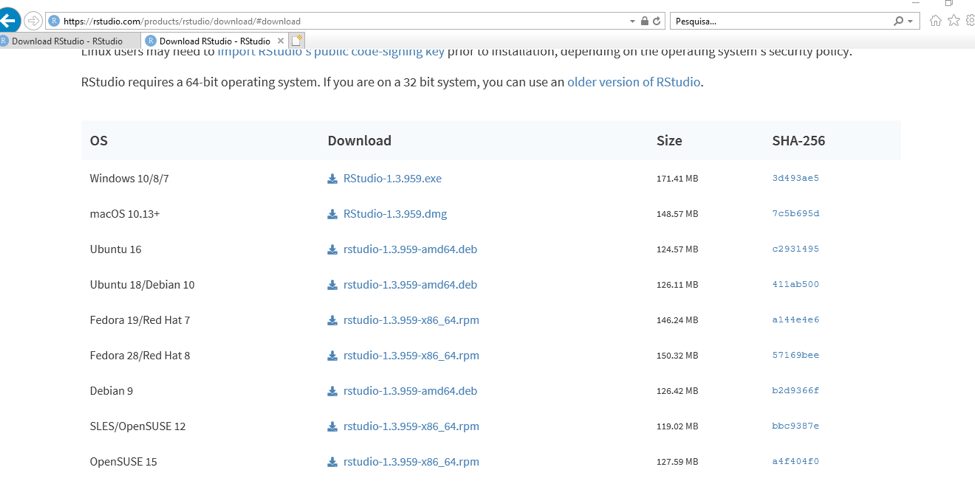
\includegraphics[width=13.54in]{img/inst_1_rstudio}

\begin{itemize}
\tightlist
\item
  Passo 3: Encontre o sistema operacional do seu computador (Ubuntu, Fedora, Debian ou OpenSUSE) e faça download.\\
\item
  Passo 4: Acesse o terminal na pasta onde foi feito o download e siga as instruções abaixo usando Fedora ou Ubuntu:

  \begin{itemize}
  \tightlist
  \item
    Fedora: \texttt{r\ sudo\ dnf\ install\ nomedo\_arquivo\_baixado.rpm}; Ex: \texttt{r\ sudo\ dnf\ install\ rstudio-1.3.959-x86\_64.rpm}
  \item
    Ubuntu: \texttt{r\ sudo\ dpkg\ -i\ nomedo\_arquivo\_baixado.deb}\\
  \end{itemize}
\item
  Passo 5: Após isso, o RStudio estará instalado no seu computador e pronto para uso.
\end{itemize}

\hypertarget{mac-os-x}{%
\section{Mac OS X}\label{mac-os-x}}

\hypertarget{instalar-o-r-1}{%
\subsection{Instalar o R}\label{instalar-o-r-1}}

\begin{itemize}
\tightlist
\item
  Passo 1: Abra o site \href{https://cran.r-project.org/}{CRAN - https://cran.r-project.org/}
\item
  Passo 2: Clique em Download de R for (Mac) OS X.\\
\item
  Passo 3: Clique duas vezes no arquivo depois de baixado que será instalado no seu computador.
\end{itemize}

\hypertarget{instalar-o-rstudio-1}{%
\subsection{Instalar o RStudio}\label{instalar-o-rstudio-1}}

\begin{itemize}
\tightlist
\item
  Passo 1: Acesse o site \url{https://rstudio.com/products/rstudio/download/}\\
\item
  Passo 2: Encontre na página o local de download gratuito conforme figura abaixo:
\end{itemize}

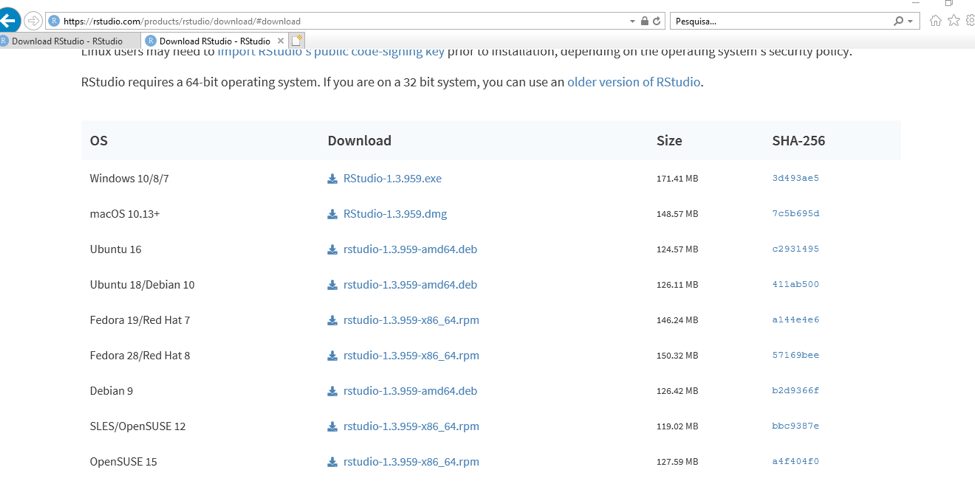
\includegraphics[width=13.54in]{img/inst_1_rstudio}

\begin{itemize}
\tightlist
\item
  Passo 3: Encontre o sistema operacional do seu computador (Mac OS) e faça download.\\
\item
  Passo 4: Depois de baixado, clique duas vezes no arquivo para instalá-lo. Após, estará pronto para uso.
\end{itemize}

\hypertarget{windows}{%
\section{Windows}\label{windows}}

\hypertarget{instalar-o-r-2}{%
\subsection{Instalar o R}\label{instalar-o-r-2}}

\begin{itemize}
\tightlist
\item
  Passo 1: Clique no seguinte link \url{https://cran.r-project.org/bin/windows/base/}\\
\item
  Passo 2: Clique em Download R for Windows (os números que aparecem nesse arquivo de download correspondem à versão do R disponível):
\end{itemize}

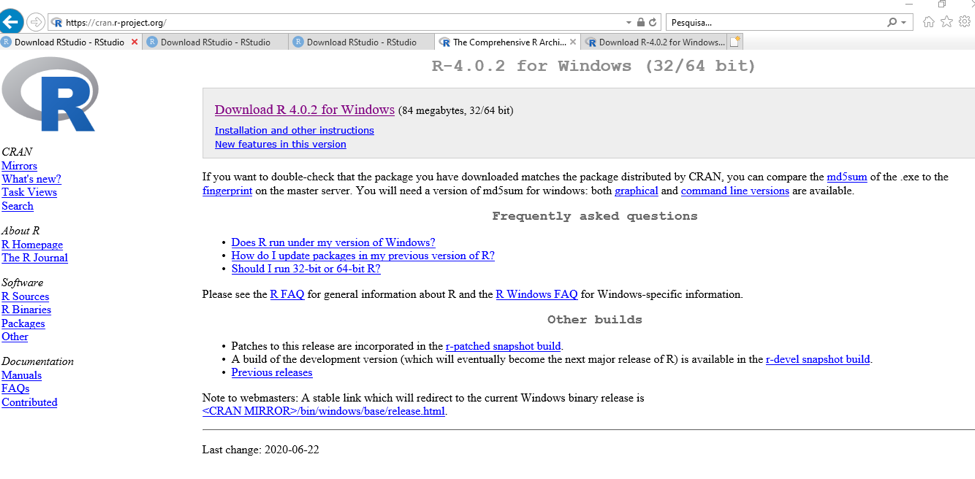
\includegraphics[width=13.54in]{img/inst_1_rwindows}

\begin{itemize}
\tightlist
\item
  Passo 3: Clique duas vezes no arquivo depois de baixado, clique em avançar até finalizar a instalação que será instalado no seu computador.
\end{itemize}

\hypertarget{instalar-o-rstudio-2}{%
\subsection{Instalar o RStudio}\label{instalar-o-rstudio-2}}

\begin{itemize}
\tightlist
\item
  Passo 1: Acesse o site \url{https://rstudio.com/products/rstudio/download/}\\
\item
  Passo 2: Encontre na página o local de download gratuito conforme figura abaixo:
\end{itemize}

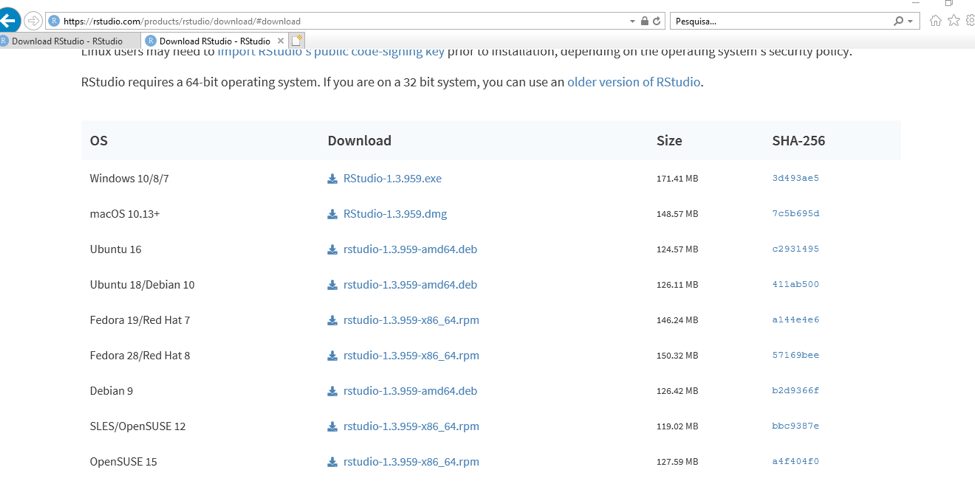
\includegraphics[width=13.54in]{img/inst_1_rstudio}

\begin{itemize}
\tightlist
\item
  Passo 3: Encontre o sistema operacional do seu computador (Windows) e faça download.
\item
  Passo 4: Depois de baixado, clique duas vezes no arquivo para instalá-lo. Após, estará pronto para uso.
\end{itemize}

\hypertarget{carregar-bibliotecas}{%
\chapter{Carregar Bibliotecas}\label{carregar-bibliotecas}}

Quando instalamos o R já dispomos de uma grande quantidades de comandos e funções. A lista de funções do R-base pode ser lida \href{https://stat.ethz.ch/R-manual/R-devel/library/base/html/00Index.html}{aqui}.

Para além destes, o ambiente R dispõe de uma grande quantidade de bibliotecas (ou pacotes) disponíveis. No momento em que escrevemos este tutorial, a plataforma de contribuições \href{https://cran.r-project.org/web/packages/}{CRAN} lista 16045 bibliotecas disponíveis. As diferentes contribuições são minimamente agrupadas por \href{https://cran.r-project.org/web/views/}{tópico}. Por exemplo, é possível conhecer os pacotes disponíveis para as \href{https://cran.r-project.org/web/views/SocialSciences.html}{ciências sociais}.

Neste tutorial vamos usar as funções do R-base e algumas bibliotecas adicionais que facilitam algumas operações e já dão conta da maior parte das necessidades de um pesquisador interessado em usar o WVS.

As bibliotecas que são usadas neste tutorial fazem parte da filosofia e gramática \href{https://www.tidyverse.org/}{tidyverse}, entre elas os pacotes \texttt{dplyr}, \texttt{haven} e \texttt{ggplot2}. Mais detalhes podem ser obtidos no livro dos autores disponível \href{https://r4ds.had.co.nz/}{neste link}. Além do \texttt{tidyverse}, usamos a biblioteca \texttt{codebook} para visualizar os dados.\footnote{Para além destas bilbiotecas usamos para compilar este tutorial as bibliotecas \texttt{bookdown}, \texttt{knitr} e \texttt{tinytex}.}

\hypertarget{instalauxe7uxe3o-de-bibliotecas-adicionais}{%
\section{Instalação de bibliotecas adicionais}\label{instalauxe7uxe3o-de-bibliotecas-adicionais}}

Como mencionamos acima, quando instalamos o R-base já instalamos uma série de funções e comandos. Dentre eles, existe um comando específico para instalar novas bibliotecas do repositório CRAN.

Para instalar as bibliotecas usa-se o comando \texttt{install.library("nome\_da\_bibliteca")}. Outra maneira de instalar novas bibliotecas é usar a aba ``Packages''. Esta aba permite visualizar as bibliotecas já instaladas e instalar novas usando o botão ``Install''.

Entrentanto, recomendamos que as bibliotecas que serão usadas nas análises sejam indicadas no inicio do código R onde são feitas as análises. Assim, o pesquisador que recebê-lo sabe quais os requisitos necessários para reproduzir as análises.

Para instalar bibliotecas adicionais, seguimos o exemplo abaixo:

\begin{Shaded}
\begin{Highlighting}[]
\CommentTok{# para instalar as bibliotecas da gramática tidyverse}
\KeywordTok{install.library}\NormalTok{(}\StringTok{"tidyverse"}\NormalTok{)}

\CommentTok{# para instalar a biblioteca codebook para visualizar os dados (ver no capítulo seguinte)}
\KeywordTok{install.library}\NormalTok{(}\StringTok{"codebook"}\NormalTok{)}
\end{Highlighting}
\end{Shaded}

Quando rodamos o comando, usando \texttt{Crtl\ +\ Enter} no script ou \texttt{Enter} diretamente no console, o R vai verificar se existem dependências e instalar todas as que forem necessárias para o seu bom funcionamento. \textbf{Assim, é importante que se faça a instalação de todas as dependências indicadas pelo R.} Verifique no console, e se o R perguntar se quer fazer a instalação das dependências, diga ``Yes''.

\hypertarget{carregar-as-bibliotecas}{%
\section{Carregar as bibliotecas}\label{carregar-as-bibliotecas}}

Uma vez instaladas as bibliotecas, é preciso carregar as bibliotecas para que possam ser usadas.

O comando para carregar as bibliotecas é \texttt{library("nome\_da\_biblioteca")}.

\begin{Shaded}
\begin{Highlighting}[]
\CommentTok{# carregar o tidyverse}
\KeywordTok{library}\NormalTok{(}\StringTok{"tidyverse"}\NormalTok{)}

\CommentTok{## carregar a biblioteca haven, que é usada no capítulo seguinte para }
\KeywordTok{library}\NormalTok{(}\StringTok{"codebook"}\NormalTok{)}

\CommentTok{# carregar o codebook}
\KeywordTok{library}\NormalTok{(}\StringTok{"codebook"}\NormalTok{)}
\end{Highlighting}
\end{Shaded}

Sempre que abrir e fechar o R-Studio é preciso carregar as bibliotecas novamente, pois o R reinicia a sessão somente com os comandos do R-base.

Carregadas as bibliotecas podemos importar os dados que vamos usar.

\hypertarget{importar-bases-de-dados}{%
\chapter{Importar bases de dados}\label{importar-bases-de-dados}}

O R importa arquivos salvos em seu próprio formato e de variados outros softwares, como Excell, SPSS e Stata, e em diversos outros formatos, incluindo Text.

Há duas formas de importação de arquivos no R: com o uso das ferramentas do Environment ou com o uso de linhas de comando escritas diretamente no console ou em um script.

\hypertarget{com-o-uso-das-ferramentas-da-aba-environment}{%
\section{Com o uso das ferramentas da aba Environment}\label{com-o-uso-das-ferramentas-da-aba-environment}}

Por esta forma, você usa as ferramentas do R do mesmo jeito que faz com qualquer outro software, como os do pacote Microsoft Office, por exemplo.

\hypertarget{arquivos-em-formato-r}{%
\subsection{Arquivos em formato R}\label{arquivos-em-formato-r}}

Para arquivos formato R (formato \texttt{.rdata}):

\begin{itemize}
\tightlist
\item
  Clique sobre o icone Abrir Arquivos.
\item
  Procure o seu arquivo nos locais do seu computador.
\item
  Clique no arquivo e clique em Open ou clique duas vezes sobre o arquivo.
\end{itemize}

Pronto! O seu arquivo vai aparecer no Environment.

\hypertarget{arquivos-em-outros-formatos}{%
\subsection{Arquivos em outros formatos}\label{arquivos-em-outros-formatos}}

Para importar os dados em outros formatos, é preciso usar biblitecas específicas para esse fim. No caso deste tutorial, a biblioteca usada é a \texttt{haven}, da gramática Tidyverse.

\begin{itemize}
\tightlist
\item
  Clique sobre o icone Import Dataset.
\item
  Escolha e clique sobre o formato em que o seu arquivo foi previamente salvo.
\item
  Clique em Browse.
\item
  Procure o seu arquivo nos locais do seu computador.
\item
  Clique no arquivo e clique em Open ou clique duas vezes sobre o arquivo.
\end{itemize}

Pronto! O seu arquivo vai aparecer no Environment.

\hypertarget{com-o-uso-de-linhas-de-comando}{%
\section{Com o uso de linhas de comando}\label{com-o-uso-de-linhas-de-comando}}

\hypertarget{arquivos-em-formato-r-1}{%
\subsection{Arquivos em formato R}\label{arquivos-em-formato-r-1}}

Para carregar arquivos no formato nativo do R usando linhas de comando:

\begin{itemize}
\tightlist
\item
  Abra um novo script R e digite: \texttt{load("nome\_do\_arquivo.rdata")}.

  \begin{itemize}
  \tightlist
  \item
    Dica: Deixe o cursor entre as aspas e tecle TAB. O R vai lhe mostrar os locais do seu computador. Se seu arquivo está em alguma pasta ou subpasta o R também vai lhe mostrar os locais do seu computador.
  \end{itemize}
\item
  Clique no arquivo que você quer importar
\item
  Digite Control + Enter, ou clique em Run (disponível na aba superior do Source Code do seu R).
\end{itemize}

Pronto! O seu arquivo vai aparecer no Environment.

\hypertarget{arquivos-em-outros-formatos-1}{%
\subsection{Arquivos em outros formatos}\label{arquivos-em-outros-formatos-1}}

Para carregar arquivos em outros formatos, usamos a biblioteca \texttt{haven} do tidyverse (Certifique-se que ela foi carregada usando o comando \texttt{library(haven)}).

Cada tipo de arquivo tem um comando específico no haven. será o mesmo para qualquer origem, com alteração apenas da extensão do arquivo:

Arquivos SPSS: função \texttt{read\_sav()}
Arquivos Excel: função \texttt{read\_csv()}
Arquivos Stata: função \texttt{read\_dta()}
Arquivos SAS: função \texttt{read\_sas()}

Veja o exemplo com a extensão do SPSS (arquivos formato .sav). Para que a base se transforme em um objeto no ambiente do R, é preciso que se atribua um nome da seguinte forma:

\begin{Shaded}
\begin{Highlighting}[]
\CommentTok{# carregar a biblioteca haven}
\KeywordTok{library}\NormalTok{(haven)}

\CommentTok{# abrir usando a função e criar um objeto no ambiente R}
\NormalTok{MinhaBase_SPSS <-}\StringTok{ }\KeywordTok{read_sav}\NormalTok{(}\StringTok{"diretório_do_projeto/nome_do_arquivo.sav"}\NormalTok{)}
\end{Highlighting}
\end{Shaded}

Como das outras vezes, deixe o cursor entre as aspas e tecle TAB. O R vai lhe mostrar os locais do seu computador. Em seguida, é só clicar sobre o arquivo que você procura.

\begin{itemize}
\tightlist
\item
  Digite Control + Enter, ou
\item
  Clique em Run (disponível na aba superior do Source Code do seu R).
\end{itemize}

Pronto! O seu arquivo vai aparecer no Environment.

Com outras extensões você usará, por exemplo, read\_cvs ou read\_dta. Para mais informações acesse a \href{https://haven.tidyverse.org/}{ajuda da bibliteca haven}

\hypertarget{gerar-dicionuxe1rio-de-variuxe1veis}{%
\section{Gerar dicionário de variáveis}\label{gerar-dicionuxe1rio-de-variuxe1veis}}

Para navegar na base de dados recém importada, reconhecer as variáveis importadas e suas características, existem diveras ferramentas disponíveis.

Uma delas é o pacote codebook, que gera um dicionário de variáveis. Nos exemplos abaixo, mostramos como gerar um dicionário de variáveis estático na aba ``Preview'' e também na forma de um vetor que pode ser visualizado como uma tabela.

\begin{Shaded}
\begin{Highlighting}[]
\CommentTok{# carregar a biblioteca codebook}
\KeywordTok{library}\NormalTok{(codebook)}

\CommentTok{# gerar um dicionário de variáveis estático navegável na aba "Preview"}
\KeywordTok{label_browser_static}\NormalTok{(base_de_dados)}

\CommentTok{# gerar uma tabela com todas as variávis}
\NormalTok{dicionario <-}\StringTok{ }\KeywordTok{codebook_table}\NormalTok{(base_de_dados)}

\CommentTok{# visualizar na forma de tabela junto aos scripts R}
\KeywordTok{view}\NormalTok{(dicionario)}
\end{Highlighting}
\end{Shaded}

Feita a importação da base e com o dicionário nas mãos podemos passar a descrição, análise e visualização dos dados.

\hypertarget{descrever-e-analisar-os-dados}{%
\chapter{Descrever e Analisar os dados}\label{descrever-e-analisar-os-dados}}

Após instalar o \textbf{software}, reconhecer seu ambiente de trabalho, instalar e carregar as bibliotecas e importar os bancos, começa a verdadeira diversão: finalmente trabalhar com os dados.

O R permite que se faça desde as operações mais simples, como uma calculadora, passando pela organização e limpeza dos dados, até análises estatísticas mais avançadas.

Um excelente começo nesta empreitada é a descrição dos dados que não só garante o divertimento do pesquisador, como também permite que se façam excelentes análises e conclusões. A partir da estatística descritiva, obtém-se um conjunto de ferramentas que permitem: a) organizar os dados - agrupando, selecionando, filtrando, ordenando, criando variáveis; b) descrever e analisar os dados - resumindo-os com base em sua média, moda, mediana, cruzando e contando as variáveis, criando gráficos e tabelas. A principal função da estatística descritiva é resumir os dados e facilitar a assimilação da informação \citep{agresti_metodos_2012}.

Além da descrição dos dados, o R também oferece suporte para que sejam feitos testes estatísticos mais avançados bi e multi-variados, dentre eles correlação e regressão linear multivariada. A correlação tem por função avaliar o comportamento de duas variáveis em função uma da outra, mensurando a interdependência das mesmas e o seu grau de associação. Logo a correlação é apropriada se o seu propósito é analisar se há relação entre a variação de duas dimensões e qual a força desta relação, como por exemplo nas clássicas premissas: nível educacional e renda variam de maneira diretamente proporcional ou apoio à democracia varia de maneira inversamente proporcional a valores autoritários. A regressão linear multivariada permite estabelecer valores estimativos de uma variável dependente em relação a um conjunto de outras variáveis independentes, isto é resulta no nível de previsibilidade de uma variável em função de outras variáveis explicativas. Deste modo, este tipo de teste se aplica aos casos em que se almeja avaliar e estabelecer potencial previsibilidade de uma variável em função de outras, e não apenas comparar seus comportamentos; por exemplo prevendo a taxa de desconfiança em relação aos partidos com base na quantidade de pessoas que estão satisfeitas com a democracia.

Nesta seção iremos aprender, então, os comandos do R que permitem criar anotações, criar variáveis e vetores, conectar sentenças do código de programação, visualizar os valores máximo e mínimo de uma variável, obter a média, somar os valores de uma variável, filtrar, selecionar, ordenar, contar, cruzar, criar nova coluna, resumir os dados a partir de alguma operação, excluir valores da análise, visualizar variáveis, fazer gráficos, fazer teste de correlação e análise de regressão multivariada. Ou seja, tudo o que se precisa para, em ordem de importância: ter adoráveis momentos com o seu banco de dados e construir conhecimento a partir de análises robustas.

\hypertarget{descrevendo-os-dados}{%
\section{Descrevendo os dados}\label{descrevendo-os-dados}}

\hypertarget{criar-variuxe1veis-e-vetores}{%
\subsection{Criar variáveis e vetores}\label{criar-variuxe1veis-e-vetores}}

Para criar uma variável basta escolher um nome para ela e atribuir através do sinal `\textless-' um valor para a mesma, lembrando sempre de que o R não aceita caractere do tipo espaço, então se o nome de sua variável tiver mais de um termo é necessário usar o conector underline `\_' entre as palavras. Para criar vetores, segue-se a mesma lógica, mas os valores devem ser inseridos entre os parênteses do código: `c()', para indicar que há um conjunto de valores; estes valores devem ser separados por vírgulas. Os valores atribuídos podem ser números simples, podem ser operações como soma, subtração, multiplicação. As variáveis e vetores, após criados podem também ter seus valores submetidos a algum tipo de operação. Exemplos:

\begin{Shaded}
\begin{Highlighting}[]
\CommentTok{# Criar um vetor com base em um resultado de cálculo}
\NormalTok{Meu_resultado <-}\StringTok{ }\DecValTok{1} \OperatorTok{+}\StringTok{ }\DecValTok{5}

\CommentTok{# Criar um vetor e multiplicar por um valor}
\NormalTok{Brasil <-}\StringTok{ }\KeywordTok{c}\NormalTok{(}\DecValTok{1}\NormalTok{, }\DecValTok{3}\NormalTok{, }\DecValTok{10}\NormalTok{, }\DecValTok{12}\NormalTok{, }\DecValTok{19}\NormalTok{, }\DecValTok{21}\NormalTok{, }\DecValTok{28}\NormalTok{, }\DecValTok{30}\NormalTok{, }\DecValTok{37}\NormalTok{)}
\NormalTok{Brasil }\OperatorTok{*}\StringTok{ }\DecValTok{3}

\CommentTok{# Cálculo da idade com base no ano de nascimento}
\NormalTok{Ano_Nasc <-}\StringTok{ }\KeywordTok{c}\NormalTok{(}\DecValTok{1990}\NormalTok{, }\DecValTok{1984}\NormalTok{, }\DecValTok{1961}\NormalTok{)}
\DecValTok{2020} \OperatorTok{-}\StringTok{ }\NormalTok{Ano_Nasc}
\NormalTok{Idade <-}\StringTok{ }\DecValTok{2020} \OperatorTok{-}\StringTok{ }\NormalTok{Ano_Nasc}
\end{Highlighting}
\end{Shaded}

\hypertarget{funuxe7uxf5es-buxe1sicas}{%
\subsection{Funções básicas}\label{funuxe7uxf5es-buxe1sicas}}

Após carregar seu banco de dados ou criar suas próprias variáveis é possível começar a conhecer e operar os dados observando seus valores máximos, mínimos, média e efetuando operações a partir dos valores dentro da variável. Para executar tais funções, os comandos são os seguintes para a variável ``Idade'':

\begin{itemize}
\tightlist
\item
  Valor máximo: \texttt{max(Idade)}
\item
  Valor mínimo: \texttt{min(Idade)}
\item
  Média: \texttt{mean(Idade)}
\item
  Soma: \texttt{sum(Idade)}
\end{itemize}

\hypertarget{estatuxedstica-descritiva}{%
\section{Estatística descritiva:}\label{estatuxedstica-descritiva}}

Partindo para funções mais sofisticadas, é possível organizar o banco de dados de maneira sistemática e fazer análises resumidas das variáveis. O comando \texttt{filter()} filtra as observações (linhas) baseadas em uma condição determinada pelo pesquisador, como por exemplo selecionar apenas determinados países, gênero feminino ou masculino, faixas de renda, idade e escolaridade.

Com o comando \texttt{select()} é possível escolher as variáveis específicas (colunas) com que se deseja trabalhar. O comando mutate cria uma nova variável (coluna) ou modifica uma já existente a partir de manipulações dos dados.

A função \texttt{count()} é muito interessante porque permite que se faça análises dos dados ao apresentar sua contagem (frequência) e cruzar variáveis.

Para agrupar conjuntos específicos de variáveis, utiliza-se o \texttt{group()}.

Outra forma de manipular e avaliar os dados é utilizando o comando \texttt{summarise()} para resumir os dados em função de alguma operação (média/mean e mediana/median).

O comando \texttt{arrange()} ordena os resultados. Outros dois comandos importantes neste contexto é o \texttt{na.rm\ =\ TRUE} para excluir missing values e o \texttt{view()} para fazer uma visualização simples de variáveis específicas.

Para exibir os dados em uma tabela, utiliza-se o comando \texttt{table()}. A seguir um resumo com o código que deve ser utilizado para executar cada uma destas funções e exemplos a partir das variáveis da base de dados do WVS:

\begin{Shaded}
\begin{Highlighting}[]
\CommentTok{# filter(), exemplo filtrar observações baseado em uma condicao Brasil: }
\KeywordTok{filter}\NormalTok{(S003 }\OperatorTok{==}\StringTok{ }\DecValTok{76}\NormalTok{)}

\CommentTok{# select(), exemplo selecionar somente país e sexo: }
\KeywordTok{select}\NormalTok{(S003, X001)}

\CommentTok{#count(), exemplo contar e cruzar as variáveis país e apoio à democracia: }
\KeywordTok{count}\NormalTok{ (S003, E235) }

\CommentTok{# mutate(), criar uma variável faixas etárias: }
\KeywordTok{mutate}\NormalTok{(}\DataTypeTok{faixa_et =} \KeywordTok{if_else}\NormalTok{(X003}\OperatorTok{<}\DecValTok{30}\NormalTok{, }\StringTok{"Jovem"}\NormalTok{, }\StringTok{"Não Jovem"}\NormalTok{))}
\end{Highlighting}
\end{Shaded}

A função `if\_else' divide os valores em dois grupos: os que se encaixam na condição e os que não se encaixam, no caso do exemplo os que possuem idade inferior a 30 (X003\textless30) é classificado como Jovem, os que não possuem são classificados como Não Jovem.

\begin{Shaded}
\begin{Highlighting}[]
\CommentTok{# summarise(), exemplo resumir os dados pela média e mediana de idade }
\KeywordTok{summarise}\NormalTok{(}\DataTypeTok{media =} \KeywordTok{mean}\NormalTok{(X003), }\DataTypeTok{mediana =} \KeywordTok{median}\NormalTok{(X003))}

\CommentTok{# para excluir missing values: na.rm = TRUE}
\NormalTok{media =}\StringTok{ }\KeywordTok{mean}\NormalTok{(X003, }\DataTypeTok{na.rm =} \OtherTok{TRUE}\NormalTok{)}

\CommentTok{# arrange(), exemplo ordenar a variável idade: }
\KeywordTok{arrange}\NormalTok{(X003)}

\CommentTok{# view(), exemplo visualizar a variável países: }
\KeywordTok{view}\NormalTok{(S003)}

\CommentTok{# table(), exemplo visualizar em uma tabela a variável faixa_et: }
\KeywordTok{table}\NormalTok{(faixa)}
\end{Highlighting}
\end{Shaded}

\hypertarget{comandos-uxfateis}{%
\subsection{Comandos úteis}\label{comandos-uxfateis}}

Para executar mais de um comando é necessário inserir entre eles o conector \texttt{\%\textgreater{}\%}. Além disso, pode ser útil acrescentar anotações que não sejam reconhecidas pelo programa como uma linha de código, para tanto basta inserir no início da frase o caractere jogo da velha \texttt{\#}.

\begin{Shaded}
\begin{Highlighting}[]
\CommentTok{# Criar anotações: #}
\CommentTok{# Conectar as linhas do código: %>% }
\CommentTok{# Exemplos: }

\NormalTok{df_wvs7 }\OperatorTok\StringTok{ }
\StringTok{  }\KeywordTok{summarise}\NormalTok{(}\DataTypeTok{media =} \KeywordTok{mean}\NormalTok{(X003, }\DataTypeTok{na.rm =} \OtherTok{TRUE}\NormalTok{)) }\OperatorTok
\StringTok{  }\KeywordTok{count}\NormalTok{(S003, X001)}
\end{Highlighting}
\end{Shaded}

\hypertarget{anuxe1lises-bi-e-multivariadas}{%
\section{Análises bi e multivariadas:}\label{anuxe1lises-bi-e-multivariadas}}

As análises descritivas oferecem diversas possibilidades para conhecer o comportamentos, distribuição e padrões das diferentes variáveis, contudo quando o objetivo é estabelecer relação entre as mesmas é necessário adotar testes mais avançados bi e multivariados. Para avaliar a taxa de associação entre duas variáveis e a capacidade explicativa de um conjunto de variáveis sobre uma variável dependente específica, devemos utilizar respectivamente correlação e regressão linear multivariada.

\hypertarget{correlauxe7uxe3o}{%
\subsection{Correlação}\label{correlauxe7uxe3o}}

Para fazer o teste de correlação basta selecionar o par de variáveis em questão e adicionar o comando \texttt{cor()} utilizando todas as observações, como no exemplo abaixo:

\begin{Shaded}
\begin{Highlighting}[]
\CommentTok{# Selecionar duas variáveis e extrair a correlação}
\NormalTok{df_wvs7 }\OperatorTok
\StringTok{  }\KeywordTok{select}\NormalTok{(X002, X003) }\OperatorTok\StringTok{ }
\StringTok{  }\KeywordTok{cor}\NormalTok{(}\DataTypeTok{use =} \StringTok{"complete.obs"}\NormalTok{)}
\end{Highlighting}
\end{Shaded}

\hypertarget{regressao-linear-multipla}{%
\section{Regressao linear multipla}\label{regressao-linear-multipla}}

Para efetuar o teste de regressão linear múltipla basta atribuir a uma variável resultado \texttt{\textless{}-} a função \texttt{lm()}.

Exemplo:

\texttt{lm(variável\ dependente\ \textasciitilde{}\ scale\ (variável\ independente\ 1)\ +\ scale\ (variável\ independente\ 2)\ +\ scale\ (variável\ independente\ n),\ data\ =.)}

É necessário sinalizar antes para o programa qual é o banco pelo nome do objeto e o recorte através das funções \texttt{group\_by()} ou \texttt{filter()}. Nos exemplos a seguir é possível visualizar melhor a estrutura do comando:

\begin{Shaded}
\begin{Highlighting}[]
\CommentTok{# Exemplos de regressão linear}
\CommentTok{# Exemplo 1: }
\NormalTok{resultado <-}\StringTok{ }\NormalTok{df_wvs7 }\OperatorTok\StringTok{ }
\StringTok{  }\KeywordTok{group_by}\NormalTok{(S003) }\OperatorTok\StringTok{ }
\StringTok{  }\KeywordTok{lm}\NormalTok{(X047 }\OperatorTok{~}\StringTok{ }\NormalTok{X025R }\OperatorTok{+}\StringTok{ }\NormalTok{X002, }\DataTypeTok{data =}\NormalTok{ .) }

\CommentTok{# Neste exemplo o "." indica que a base de dados é enviada na função lm() depois do "e então" %>% }

\CommentTok{# Exemplo 2: }
\NormalTok{resultado_bol <-}\StringTok{ }\NormalTok{df_wvs7 }\OperatorTok\StringTok{ }
\StringTok{  }\KeywordTok{filter}\NormalTok{(S003 }\OperatorTok{==}\StringTok{ }\DecValTok{68}\NormalTok{) }\OperatorTok\StringTok{ }
\StringTok{  }\KeywordTok{lm}\NormalTok{(X047 }\OperatorTok{~}\StringTok{ }\KeywordTok{scale}\NormalTok{(X025R) }\OperatorTok{+}\StringTok{ }\KeywordTok{scale}\NormalTok{(X002), }\DataTypeTok{data =}\NormalTok{ .)}

\CommentTok{# Neste exemplo as variáveis são normalizadas com a função scale() e foi filtrado apenas o país código 68. }
\end{Highlighting}
\end{Shaded}

\hypertarget{visualizar-os-dados}{%
\chapter{Visualizar os dados}\label{visualizar-os-dados}}

Para visualizar os dados, usamos a biblioteca \texttt{ggplot2()} também da gramática Tidyverse.

Após organizar e manipular os dados e fazer análises descritivas, pode ser uma boa estratégia apresentar as informações em gráficos para evidenciar padrões, tendências e comparações. Conforme visto anteriormente, a biblioteca para plotar gráficos é a \texttt{ggplot()}. A biblioteca \texttt{ggthemes()} permite aplicar alguns temas já pré-estabelecidos.

O \texttt{ggplot} é uma biblioteca que constrói os gráficos em camadas. Primeiramente se define a ``folha'' com uma base de dados que será usada. Em seguida a geometria que será usada e os demais parâmetros dos gráficos.

O comando básico do ggplot é: \texttt{ggplot(data\ =\ dados,\ aes(x\ =\ Explicativa,\ y\ =\ Resposta))\ +\ geoma\ +\ ...}

Tipos de Geomas disponíveis:

\begin{itemize}
\tightlist
\item
  Histograma: \texttt{geom\_hist()}
\item
  Barras: \texttt{geom\_bar()}
\item
  Pontos: \texttt{geom\_point()}
\item
  Diagrama de caixa (boxplot): \texttt{geom\_boxplot()}
\item
  Linhas: \texttt{geom\_line()}
\end{itemize}

O guia do ggplot2 pode ser encontrado \href{https://ggplot2.tidyverse.org/index.html}{aqui}. Nesta \href{https://www.r-graph-gallery.com/}{galeria} podem ser encontrados diversos exemplos de gráficos para se inspirar.

\begin{Shaded}
\begin{Highlighting}[]
\CommentTok{# Exemplo 1 plotar um gráfico de densidade da variável idade: }
\KeywordTok{ggplot}\NormalTok{(df_wvs7, }\KeywordTok{aes}\NormalTok{(}\DataTypeTok{x =}\NormalTok{ X003)) }\OperatorTok{+}\StringTok{ }\KeywordTok{geom_density}\NormalTok{() }
\end{Highlighting}
\end{Shaded}

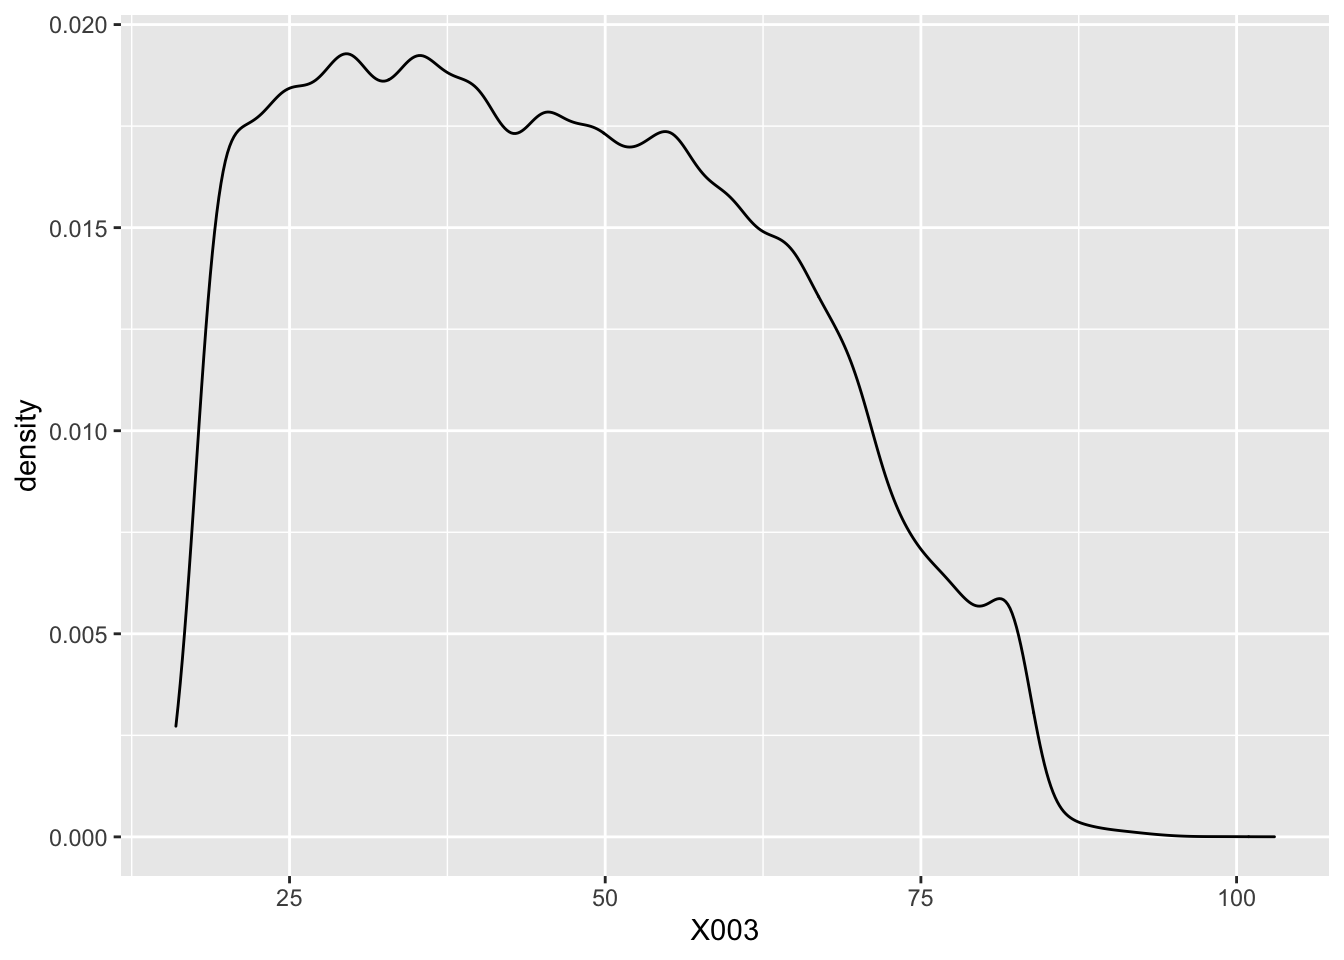
\includegraphics{tiagovier.github.io_files/figure-latex/densidade-1.pdf}

No exemplo abaixo, reproduzimos o mapa cultural do Inglehart \citep{inglehart_modernization_2005} para alguns paíse. Mas antes é preciso fazer algumas manipulações com os dados com o que aprendemos nos capítulos anteriores.

\begin{Shaded}
\begin{Highlighting}[]
\CommentTok{# Criar uma lista com os países que se quer analisar}
\NormalTok{paises <-}\StringTok{ }\KeywordTok{c}\NormalTok{(}\DecValTok{76}\NormalTok{, }\DecValTok{32}\NormalTok{, }\DecValTok{152}\NormalTok{, }\DecValTok{170}\NormalTok{) }\CommentTok{# 76=Brasil, 32=Chile, 152=Argentina, 170=Colombia }

\CommentTok{# Extrair e retrabalhar as variáveis que precisamos}
\NormalTok{df_y001 <-}\StringTok{ }\NormalTok{df_wvs7 }\OperatorTok
\StringTok{  }\KeywordTok{select}\NormalTok{(S024, S020, S003, tradrat5, survself) }\OperatorTok\StringTok{ }\CommentTok{# selecionar as variáveis de interesse}
\StringTok{  }\KeywordTok{filter}\NormalTok{(S003 }\OperatorTok\StringTok{ }\NormalTok{paises) }\OperatorTok\StringTok{ }\CommentTok{# filtrar os países}
\StringTok{  }\KeywordTok{group_by}\NormalTok{(S024, S020, S003) }\OperatorTok\StringTok{ }\CommentTok{# agrupar por onda-país, onda e país}
\StringTok{  }\KeywordTok{summarise}\NormalTok{(}\DataTypeTok{tradrat5 =} \KeywordTok{mean}\NormalTok{(tradrat5, }\DataTypeTok{na.rm =}\NormalTok{ T),}
            \DataTypeTok{survself =} \KeywordTok{mean}\NormalTok{(survself, }\DataTypeTok{na.rm =}\NormalTok{ T)) }\CommentTok{# agregar os dados pela média}
\end{Highlighting}
\end{Shaded}

Feito isso podemos criar a figura:

\begin{Shaded}
\begin{Highlighting}[]
\CommentTok{# lembre se de carregar a variável ggplot se ela não tiver sido carregada }
\KeywordTok{library}\NormalTok{(ggplot2)}

\CommentTok{# Reproduzir o Mapa Cultural Inglehart }
\KeywordTok{ggplot}\NormalTok{(df_y001, }\KeywordTok{aes}\NormalTok{(}\DataTypeTok{x =}\NormalTok{ survself, }
                    \DataTypeTok{y =}\NormalTok{ tradrat5, }
                    \DataTypeTok{color =} \KeywordTok{as.factor}\NormalTok{(S003), }
                    \DataTypeTok{label =} \KeywordTok{as.factor}\NormalTok{(S003))) }\OperatorTok{+}\StringTok{ }\CommentTok{# definir os dados e as dimensões}
\StringTok{  }\KeywordTok{geom_point}\NormalTok{() }\OperatorTok{+}\StringTok{ }\CommentTok{# definir a geometria principal (pontos)}
\StringTok{  }\KeywordTok{geom_text}\NormalTok{(}\DataTypeTok{hjust =} \DecValTok{0}\NormalTok{, }\DataTypeTok{nudge_x =} \FloatTok{0.05}\NormalTok{, }\DataTypeTok{check_overlap =} \OtherTok{TRUE}\NormalTok{) }\OperatorTok{+}\StringTok{ }\CommentTok{# adicionar os rótulos com a geometria de texto}
\StringTok{  }\KeywordTok{scale_x_continuous}\NormalTok{(}\DataTypeTok{limits =} \KeywordTok{c}\NormalTok{(}\OperatorTok{-}\DecValTok{2}\NormalTok{, }\DecValTok{2}\NormalTok{)) }\OperatorTok{+}\StringTok{ }\CommentTok{# restringir o eixo x e y entre -2 e 2}
\StringTok{  }\KeywordTok{scale_y_continuous}\NormalTok{(}\DataTypeTok{limits =} \KeywordTok{c}\NormalTok{(}\OperatorTok{-}\DecValTok{2}\NormalTok{, }\DecValTok{2}\NormalTok{)) }\OperatorTok{+}
\StringTok{  }\KeywordTok{labs}\NormalTok{(}\DataTypeTok{x =} \StringTok{"sobrevivencia-autoexpressão"}\NormalTok{,}
       \DataTypeTok{y =} \StringTok{"tradicional-racional"}\NormalTok{,}
       \DataTypeTok{title =} \StringTok{"Mapa Cultural do Inglehart (Brasil, Chile, Argentina, Colombia)"}\NormalTok{) }\CommentTok{# adicionar os rótulos x, y e título}
\end{Highlighting}
\end{Shaded}

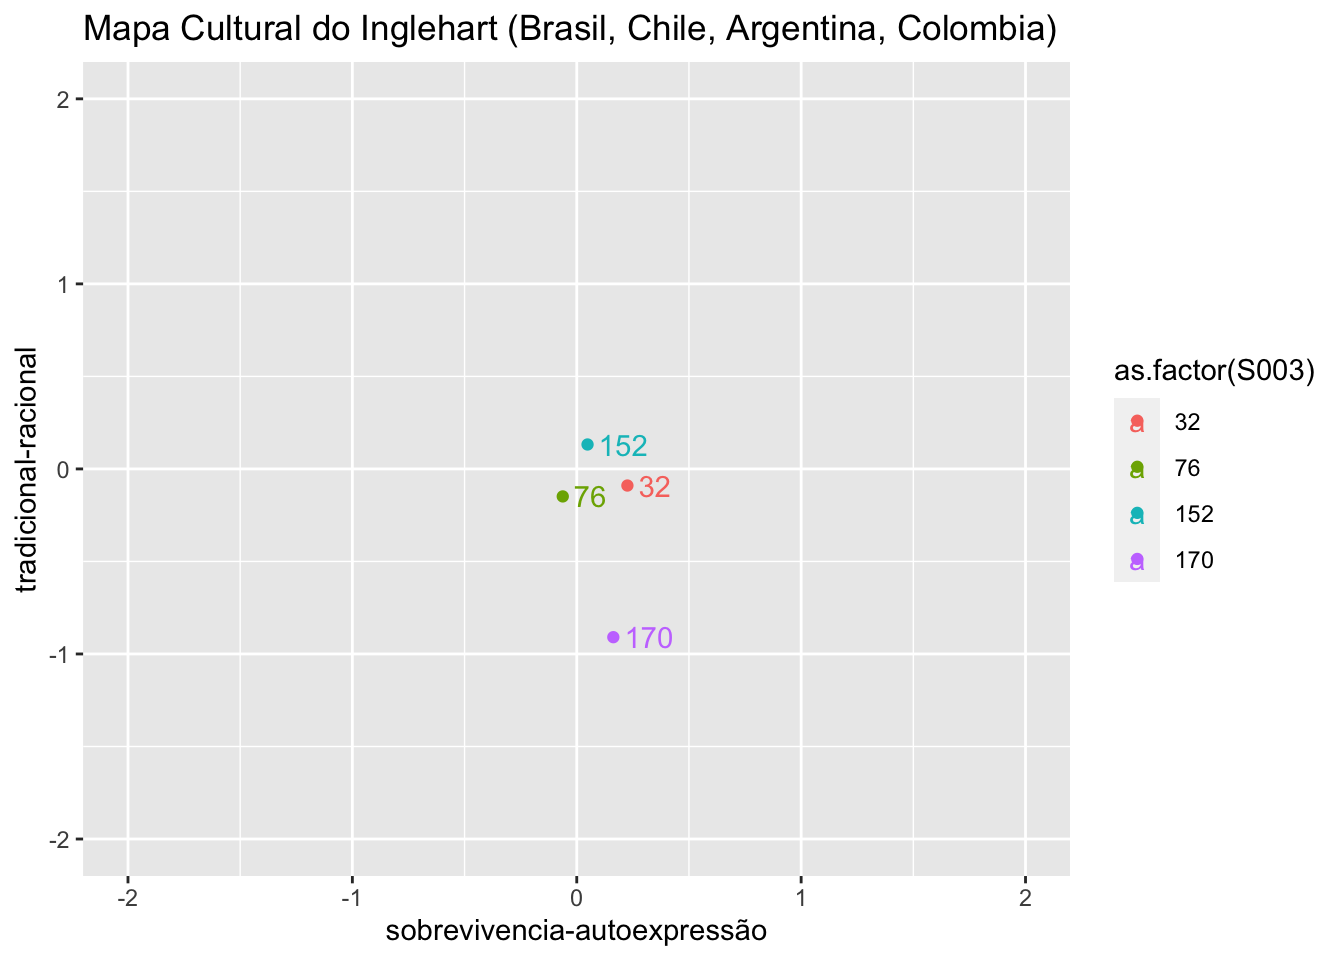
\includegraphics{tiagovier.github.io_files/figure-latex/mapacultural-1.pdf}

\hypertarget{glossuxe1rio}{%
\chapter{Glossário}\label{glossuxe1rio}}

\begin{itemize}
\tightlist
\item
  Programação: alguns conceitos relevantes para aprender uma linguagem de programação.

  \begin{itemize}
  \tightlist
  \item
    Variável: representa um local de armazenamento na memória, com um nome e um valor, mas que não é o valor em si, porque este pode ser constantemente alterado. Cada variável possui diferentes propriedades, por exemplo, pode ser numeric (números) ou string (letras). Inserindo uma metáfora: cada variável seria uma ``caixinha'' que pode guardar alguma coisa, e tem diferentes características (grande, pequena, quadrada, redonda). \texttt{x\ \textless{}-\ 2\ \#cria\ variável\ "x"\ e\ atribuir\ valor\ 2}
  \item
    Objeto: cada objeto é único, específico, e pode ser sempre referenciado. Seu conteúdo pode ser um atribuído diretamente, ou ser o resultado de uma operação. Cada objeto pode ser armazenado em uma variável. Na metáfora, um objeto pode ser uma carta, uma moeda, um lápis-de-cor. \texttt{y\ \textless{}-\ 5\ \#criar\ objeto\ com\ nome\ y\ e\ atribuir\ valor\ 5}
  \item
    Vetor: uma sequência ordenada de elementos. Importante notar que um vetor armazena apenas um ``tipo'' de informação, por exemplo, só números, o que se chama de unidimensional. Como se fosse uma caixinha com várias cartas (uma de fulano, outra de beltrano, etc), ou uma caixinha com várias moedas (1 euro, 50 centavos de dólar, 25 centavos de real, etc), ou uma caixinha com diferentes lápis-de-cor (rosa, azul, verde). \texttt{z\ \textless{}-\ c(1,\ 2,\ 3)\ \#criar\ vetor\ z\ e\ atribuir\ os\ valores\ 1,\ 2\ e\ 3}
  \item
    Lista: é como um vetor ``avançado'', pois também é uma sequência de elementos mas pode guardar diferentes tipos de dados (números, letras, etc), ou seja, é multidimensional. Assim, pode ser uma mesma caixinha que guarda, tudo junto, cartas, moedas e lápis-de-cor. \texttt{lista\ \textless{}-\ list(idade\ =\ 20,\ “oi”,\ 35,\ “tchau”)\ \#criar\ "lista"\ e\ atribuir\ diferentes\ conteúdos}
  \end{itemize}
\item
  Interfaces: o RStudio possui quatro interfaces, que são as ``pequenas telas'' ou ``janelinhas'' que aparecem ao iniciar o programa. Pensando em uma cozinha, o source seria a receita, o passo-a-passo; o console seria o fogão, onde tudo está acontecendo, onde forma o resultado; e o environment seria uma mesa, onde estão os ingredientes disponíveis. Os pacotes e arquivos são o armário com os utensílios de cozinha e ingredientes disponíveis.

  \begin{itemize}
  \tightlist
  \item
    Source: local onde são inseridos os códigos-fonte, no canto superior esquerdo.
  \item
    Console: também chamado de terminal, onde são mostrados os resultados dos comandos executados pelos códigos, no canto inferior esquerdo.
  \item
    Environment: também chamado de ambiente, onde são mostrados os elementos (por exemplo, vetores, bases de dados, etc) que foram criados, no canto superior direito.
  \item
    Viewer: também chamado files, onde são mostrados os arquivos, pacotes, pastas, entre outros, no canto inferior direito.
  \end{itemize}
\item
  Funções: diferentes ``verbos'', tanto do r-base quanto na gramática Tidyverse, realizam diferentes tipos de funções.

  \begin{itemize}
  \tightlist
  \item
    Count: conta quantas vezes aparece aquela variável, por exemplo, numa base de dados, e mostra seu valor. \texttt{count(x)\ \#contar\ a\ quantidade\ da\ variável\ x}
  \item
    Filter: filtrar observações (``cadastros'') baseadas em uma condição. \texttt{filter(x\ ==\ 1)\ \#filtra\ todos\ os\ valores\ de\ x\ e\ deixar\ apenas\ os\ cadastros\ em\ que\ x\ tem\ o\ valor\ 1}
  \item
    Select: selecionar variáveis - no plural -, ou seja, escolher mais de uma variável. \texttt{select(x,\ y,\ z)\ \#selecionar\ as\ variáveis\ x,\ y\ e\ z}
  \item
    Group\_by: agrupar variáveis, por exemplo, em uma base de dados grande, ``juntar'' a partir de um determinado quesito. \texttt{group\_by(país)\ \#juntar\ os\ dados\ com\ base\ nos\ diferentes\ valores\ da\ variável\ país}
  \item
    View: visualizar a operação realizada, normalmente, o R cria uma tabela com o(s) conteúdo(s), ficando mais ``simples'' de enxergar os dados. \texttt{view(objeto)}
  \item
    Summarise: resumir, sintetizar, os dados baseados em uma operação, ou seja, criando uma espécie de ``atalho''. \texttt{summarize(media\ =\ mean(idade))\ \#tem\ a\ média\ das\ idades\ das\ pessoas\ como\ critério\ para\ resumir\ ou\ sintetizar\ os\ dados}
  \item
    Mutate: criar nova informação com base em outras, visualmente, é como se criasse uma nova ``coluna''. \texttt{view(a\ =\ b\ +\ c)\ \#a\ ‘coluna’\ a\ vai\ ter\ o\ valor\ da\ soma\ de\ b\ e\ c}
  \end{itemize}
\item
  Códigos-chave:

  \begin{itemize}
  \tightlist
  \item
    \texttt{\#} para fazer comentários, ou seja, escrever anotações sem que elas sejam executadas como códigos.
  \item
    \texttt{\%\textgreater{}\%} para criar um comando no sentido de ``e então'', ou seja, especificar que seja realizado o próximo passo do código em seguida, dica: clicar \texttt{Ctrl\ +\ Shift\ +\ M}.
  \item
    \texttt{Ctrl\ +\ enter}, ou clicar no botão \texttt{Run}, para ``rodar'', ou seja, executar o código programado/escrito.
  \end{itemize}
\item
  Estatística:

  \begin{itemize}
  \tightlist
  \item
    Variáveis numéricas: quantitativas, podem ser discretas (contagem, ex.: número de filhos) ou contínuas (mensuração, ex.: peso, altura)
  \item
    Variáveis categóricas: qualitativas, podem ser ordinais (quando há ordem, ex.: grau de instrução) ou nominais (classificação, ex.: sexo, raça)
  \end{itemize}
\end{itemize}

  \bibliography{tutorial.bib,packages.bib}

\end{document}
